\section{Feature Attribution: SHAP and LIME}

\begin{frame}{Baseline: Permutation Importance}

    \begin{block}{Recipe}
        \begin{enumerate}
            \item Measure the model's score on the validation set.
            \item Shuffle one feature column, breaking its relationship with the target.
            \item Re-score. The \textbf{drop} is that feature's importance.
            \item Repeat several times and average; then restore the column and move on.
        \end{enumerate}
    \end{block}

    \vspace{0.7em}

    \begin{columns}[T]
        \begin{column}{0.48\textwidth}
            \textbf{Why start here}
            \begin{itemize}\small
                \setlength\itemsep{0.3em}
                \item Model-agnostic, ten lines of code, needs only \texttt{predict()}.
                \item Measures importance \textbf{for the metric you care about}.
                \item Computed on \emph{held-out} data, so it reflects generalisation, not fit.
            \end{itemize}
        \end{column}
        \begin{column}{0.48\textwidth}
            \textbf{Where it misleads}
            \begin{itemize}\small
                \setlength\itemsep{0.3em}
                \item \textbf{Correlated features split the credit}, and each looks unimportant
                      because the other covers for it.
                \item Shuffling creates impossible rows (age 8, income \$200k), so you evaluate
                      the model off its data manifold.
                \item It is global only --- it says nothing about a single prediction.
            \end{itemize}
        \end{column}
    \end{columns}
\end{frame}

\begin{frame}{A Trap: Built-in Tree ``Feature Importance''}

    \texttt{RandomForest.feature\_importances\_} is \textbf{mean decrease in impurity} (MDI),
    accumulated on the \emph{training} data.

    \vspace{0.8em}

    \begin{itemize}
        \setlength\itemsep{0.5em}
        \item It is biased towards \textbf{high-cardinality} features: a continuous feature or a
              random ID column offers many split points, so it looks informative even when it is
              pure noise.
        \item It is computed on training data, so it rewards features the model used to overfit.
        \item Classic demonstration: add a column of random integers to your dataset and it can
              outrank real predictors in MDI --- while permutation importance on held-out data
              correctly gives it roughly zero.
    \end{itemize}

    \vspace{0.8em}
    \begin{block}{}
        \centering
        \small Rule: never report \texttt{feature\_importances\_} as ``the model's feature
        importance'' without saying which definition you used. Prefer permutation importance
        or SHAP on held-out data.
    \end{block}
\end{frame}

\begin{frame}{SHAP: Attribution as a Fair Payout}

    \textbf{The analogy.} A team of players cooperates and earns a payout. How much of it does each
    player deserve? Here the ``players'' are the features of one row, and the ``payout'' is
    $f(x) - \mathbb{E}[f(X)]$: how far this prediction sits from the average prediction.

    \vspace{0.8em}

    \begin{block}{Shapley value (Shapley, 1953)}
        Consider adding feature $i$ to a coalition $S$ of features already present, and record the
        change in the prediction. The Shapley value $\phi_i$ is the \textbf{average of that change
        over all possible orderings} in which features could be added:
        \[
            \phi_i \;=\; \sum_{S \subseteq N \setminus \{i\}}
            \frac{|S|!\,\bigl(|N|-|S|-1\bigr)!}{|N|!}
            \Bigl[\, v(S \cup \{i\}) - v(S) \,\Bigr]
        \]
    \end{block}

    \vspace{0.5em}

    \begin{itemize}\small
        \setlength\itemsep{0.3em}
        \item The averaging over orderings is what makes it symmetric: no feature is privileged by
              being ``first''.
        \item There are $2^{|N|}$ subsets, so the exact computation is exponential.
              Everything practical in SHAP is an efficient approximation of this quantity.
    \end{itemize}
\end{frame}

\begin{frame}[allowframebreaks]{Why This Particular Formula: The Axioms}

    Lundberg and Lee (2017) define a class of \emph{additive feature attribution} methods and show
    that within it exactly \textbf{one} solution satisfies three properties --- the Shapley values.
    They also show that several earlier methods (LIME with a particular kernel, DeepLIFT,
    layer-wise relevance propagation) are members of that same class.

    \vspace{0.8em}

    \begin{itemize}
        \setlength\itemsep{0.5em}
        \item \textbf{Local accuracy (efficiency).} The parts add up to the whole:
              \[
                  f(x) \;=\; \underbrace{\mathbb{E}[f(X)]}_{\text{base value}} \;+\; \sum_{i} \phi_i
              \]
              This is what makes a SHAP plot readable: the bars literally sum to the prediction.
        \item \textbf{Missingness.} A feature that is absent from the model gets $\phi_i = 0$.
        \item \textbf{Consistency.} If you change the model so that a feature's marginal
              contribution never decreases, its attribution cannot decrease. Common tree importance
              measures (gain, split count) violate this --- the formal reason to prefer SHAP for
              tree models.
    \end{itemize}

    \vspace{0.3em}
    {\scriptsize S.~M.~Lundberg and S.-I.~Lee, ``A Unified Approach to Interpreting Model
    Predictions,'' NeurIPS 2017, \href{https://arxiv.org/abs/1705.07874v2}{arXiv:1705.07874v2}.}
\end{frame}

\begin{frame}{What SHAP Consumes and Produces}

    \centering
    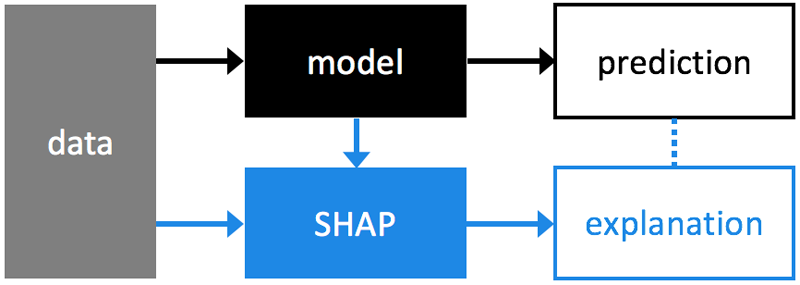
\includegraphics[width=0.50\textwidth,height=0.34\textheight,keepaspectratio]{images/responsible-ai/shap_pipeline_diagram.png}

    \vspace{0.3em}
    {\scriptsize Source: \texttt{shap} library documentation artwork,
    \href{https://github.com/shap/shap}{github.com/shap/shap} (\texttt{docs/artwork/shap\_diagram.png}).}

    \vspace{0.7em}
    \raggedright
    \begin{itemize}\small
        \setlength\itemsep{0.3em}
        \item SHAP does not change the model. It takes the \textbf{fitted model} plus a
              \textbf{background dataset} and produces one attribution per feature per row.
        \item The background dataset defines $\mathbb{E}[f(X)]$ --- the reference the explanation is
              measured against. \textbf{Change the background and every number changes}, so record
              which rows you used.
        \item A useful phrasing for stakeholders: \emph{``compared with a typical applicant, this
              applicant's income pushed the score up by 0.31.''}
    \end{itemize}
\end{frame}

\begin{frame}{Local View: The Waterfall Plot}

    \centering
    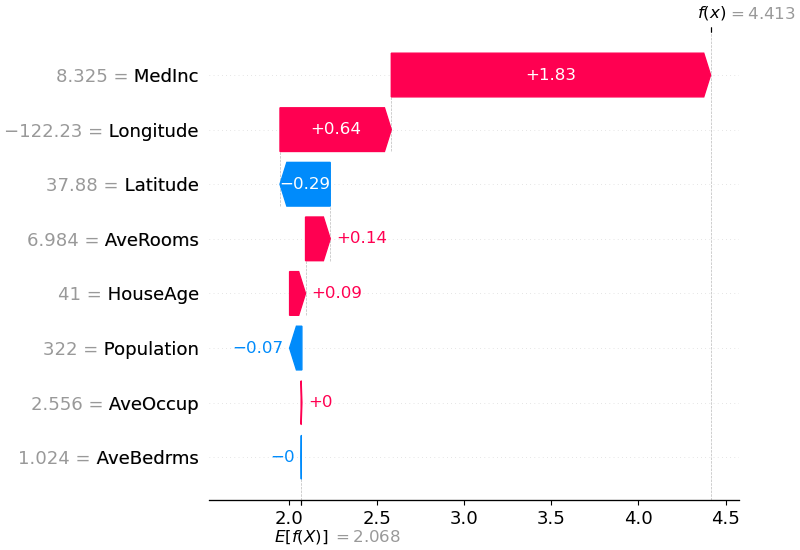
\includegraphics[width=0.60\textwidth,height=0.42\textheight,keepaspectratio]{images/responsible-ai/shap_waterfall_california.png}

    \vspace{0.3em}
    {\scriptsize Source: \texttt{shap} library documentation artwork,
    \href{https://github.com/shap/shap}{github.com/shap/shap}
    (\texttt{docs/artwork/california\_waterfall.png}); model trained on the California Housing
    dataset, target in units of \$100k.}

    \vspace{0.6em}
    \raggedright
    \begin{itemize}\small
        \setlength\itemsep{0.3em}
        \item Read bottom to top: start at the base value $\mathbb{E}[f(X)] = 2.068$, add each
              feature's contribution, arrive at this row's prediction $f(x) = 4.413$.
        \item The grey number on the left is the feature's actual value for this row.
        \item This is the artefact to show a domain expert. One row, one story, and it adds up.
    \end{itemize}
\end{frame}

\begin{frame}{Global View: The Beeswarm Summary Plot}

    \centering
    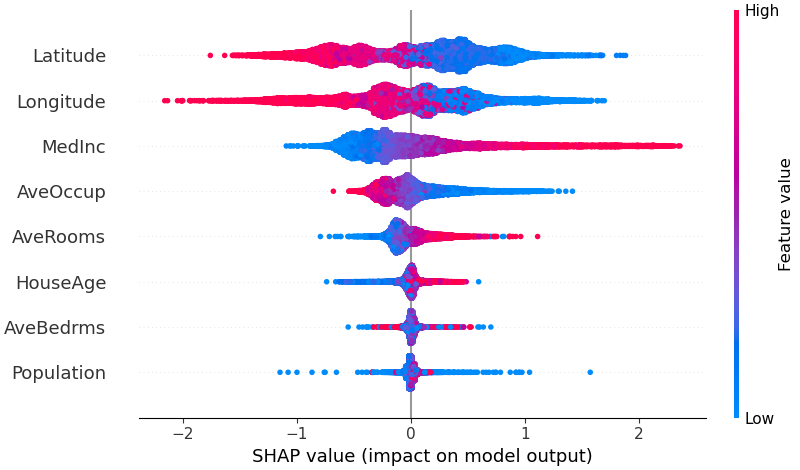
\includegraphics[width=0.58\textwidth,height=0.42\textheight,keepaspectratio]{images/responsible-ai/shap_beeswarm_california.png}

    \vspace{0.3em}
    {\scriptsize Source: \texttt{shap} library documentation artwork,
    \href{https://github.com/shap/shap}{github.com/shap/shap}
    (\texttt{docs/artwork/california\_beeswarm.png}).}

    \vspace{0.5em}
    \raggedright
    \begin{itemize}\small
        \setlength\itemsep{0.3em}
        \item One dot per row per feature; horizontal position is the SHAP value, colour is the
              \textbf{feature value} (red high, blue low). Features are ordered by mean $|\phi|$.
        \item Read the \textbf{direction}: for \texttt{MedInc}, red dots sit on the right, so higher
              median income pushes the predicted price up --- monotone and sensible.
        \item Read the \textbf{spread}: a feature with a wide swarm matters a lot for some rows and
              not at all for others. A bar chart of mean $|\phi|$ would have hidden that.
    \end{itemize}
\end{frame}

\begin{frame}{Interaction View: The Dependence / Scatter Plot}

    \centering
    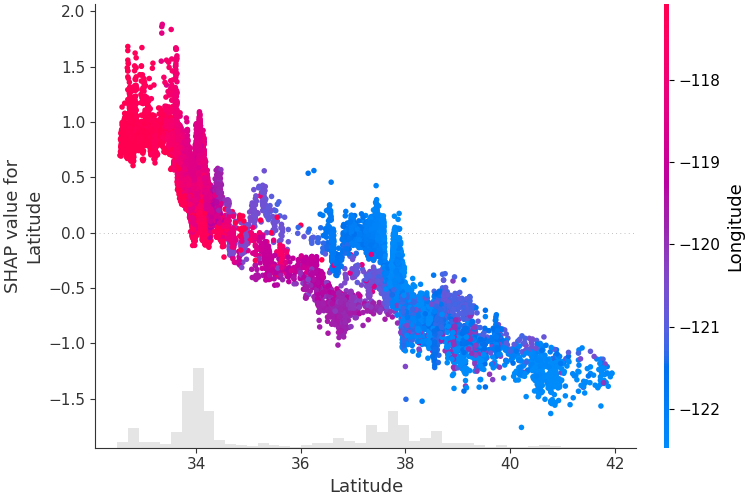
\includegraphics[width=0.47\textwidth,height=0.42\textheight,keepaspectratio]{images/responsible-ai/shap_scatter_california.png}

    \vspace{0.3em}
    {\scriptsize Source: \texttt{shap} library documentation artwork,
    \href{https://github.com/shap/shap}{github.com/shap/shap}
    (\texttt{docs/artwork/california\_scatter.png}).}

    \vspace{0.5em}
    \raggedright
    \begin{itemize}\small
        \setlength\itemsep{0.3em}
        \item $x$-axis: the feature's value. $y$-axis: its SHAP value. This is the model's learned
              response to that feature, without assuming it is linear or monotone.
        \item Colouring by a second feature exposes \textbf{interactions}: here the vertical spread
              at a given latitude is explained by longitude --- the model has learned geography,
              not a one-dimensional rule.
        \item Sharp steps are informative: they are the split points of the underlying trees.
    \end{itemize}
\end{frame}

\begin{frame}{Which SHAP Estimator?}

    \centering
    \scriptsize
    \begin{tabular}{p{2.5cm} p{4.2cm} p{5.2cm}}
        \toprule
        \textbf{Estimator} & \textbf{Applies to} & \textbf{Notes} \\
        \midrule
        \textbf{TreeSHAP} & Trees, random forests, gradient boosting (XGBoost, LightGBM, CatBoost)
        & Exact, in polynomial time, by exploiting the tree structure. Fast enough for a whole
          dataset. \textbf{Use this whenever you can.} \\
        \addlinespace
        \textbf{KernelSHAP} & Anything with \texttt{predict()}
        & Weighted local linear regression over sampled coalitions. Model-agnostic but
          \textbf{slow}; sample a few hundred background rows and a subset of instances. \\
        \addlinespace
        \textbf{DeepSHAP / Gradient} & Neural networks
        & Uses backpropagation and a DeepLIFT-style approximation; much cheaper than KernelSHAP. \\
        \addlinespace
        \textbf{Linear} & Linear models
        & Closed form: $\phi_i = w_i (x_i - \mathbb{E}[X_i])$ under feature independence. \\
        \bottomrule
    \end{tabular}

    \vspace{0.9em}
    \raggedright
    {\scriptsize Polynomial-time exact tree attribution: S.~M.~Lundberg et al., ``From local
    explanations to global understanding with explainable AI for trees,'' \emph{Nature Machine
    Intelligence} 2:56--67, 2020.}
\end{frame}

\begin{frame}{LIME: Fit a Simple Model in a Small Neighbourhood}

    \centering
    \resizebox{\textwidth}{!}{%
    \begin{tikzpicture}[
        node distance=0.75cm,
        limestep/.style={rectangle, draw, rounded corners, minimum height=1.25cm, text width=2.35cm,
                     align=center, font=\scriptsize, fill=raiBlue!10},
        arr/.style={-{Latex[length=2.2mm]}, thick}
    ]
        \node[limestep] (a) {Pick the row $x$ to explain};
        \node[limestep, right=of a] (b) {Perturb it: sample many nearby variants};
        \node[limestep, right=of b] (c) {Ask the black box to label them};
        \node[limestep, right=of c] (d) {Weight samples by closeness to $x$};
        \node[limestep, right=of d, fill=raiGreen!12] (e) {Fit a sparse linear model on the weights};

        \foreach \x/\y in {a/b, b/c, c/d, d/e} \draw[arr] (\x) -- (\y);
    \end{tikzpicture}}

    \vspace{1.0em}

    \raggedright
    \begin{itemize}
        \setlength\itemsep{0.4em}
        \item The coefficients of that little linear model \emph{are} the explanation.
        \item ``Perturb'' is domain-specific: for text, delete words; for images, switch
              superpixels on and off; for tabular data, sample around the row.
        \item The surrogate is deliberately \textbf{sparse} (a handful of features) so a human can
              read it. Complexity is traded for legibility, on purpose.
    \end{itemize}

    \vspace{0.4em}
    {\scriptsize M.~T.~Ribeiro, S.~Singh and C.~Guestrin, ``\,`Why Should I Trust You?': Explaining
    the Predictions of Any Classifier,'' KDD 2016,
    \href{https://arxiv.org/abs/1602.04938v3}{arXiv:1602.04938v3}.}
\end{frame}

\begin{frame}{LIME on Tabular Data}

    \centering
    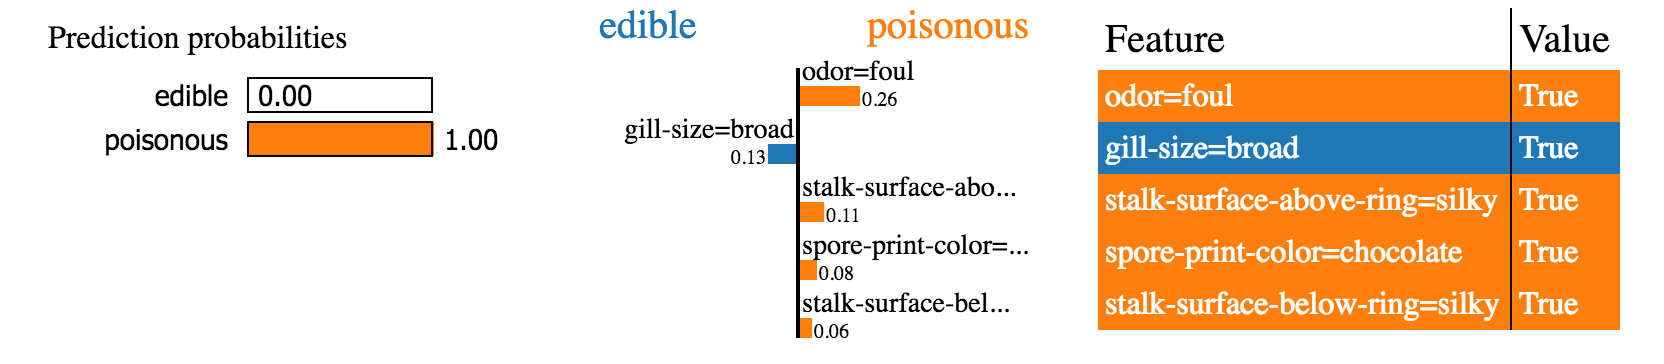
\includegraphics[width=0.92\textwidth,height=0.40\textheight,keepaspectratio]{images/responsible-ai/lime_tabular_explanation.png}

    \vspace{0.3em}
    {\scriptsize Source: \texttt{lime} library documentation,
    \href{https://github.com/marcotcr/lime}{github.com/marcotcr/lime}
    (\texttt{doc/images/tabular.png}); mushroom edibility classifier.}

    \vspace{0.7em}
    \raggedright
    \begin{itemize}\small
        \setlength\itemsep{0.3em}
        \item Left: the predicted class probabilities. Middle: signed contributions of the top
              features. Right: the actual feature values for this row.
        \item The explanation is in terms of \textbf{discretised bins}
              (\texttt{odor=foul}), which is why it reads well to a non-specialist --- and why the
              numbers depend on how you binned.
        \item Note the contrast with SHAP: LIME's weights are coefficients of a local surrogate.
              They do \textbf{not} sum to the prediction.
    \end{itemize}
\end{frame}

\begin{frame}{LIME on Text: Finding a Shortcut}

    \centering
    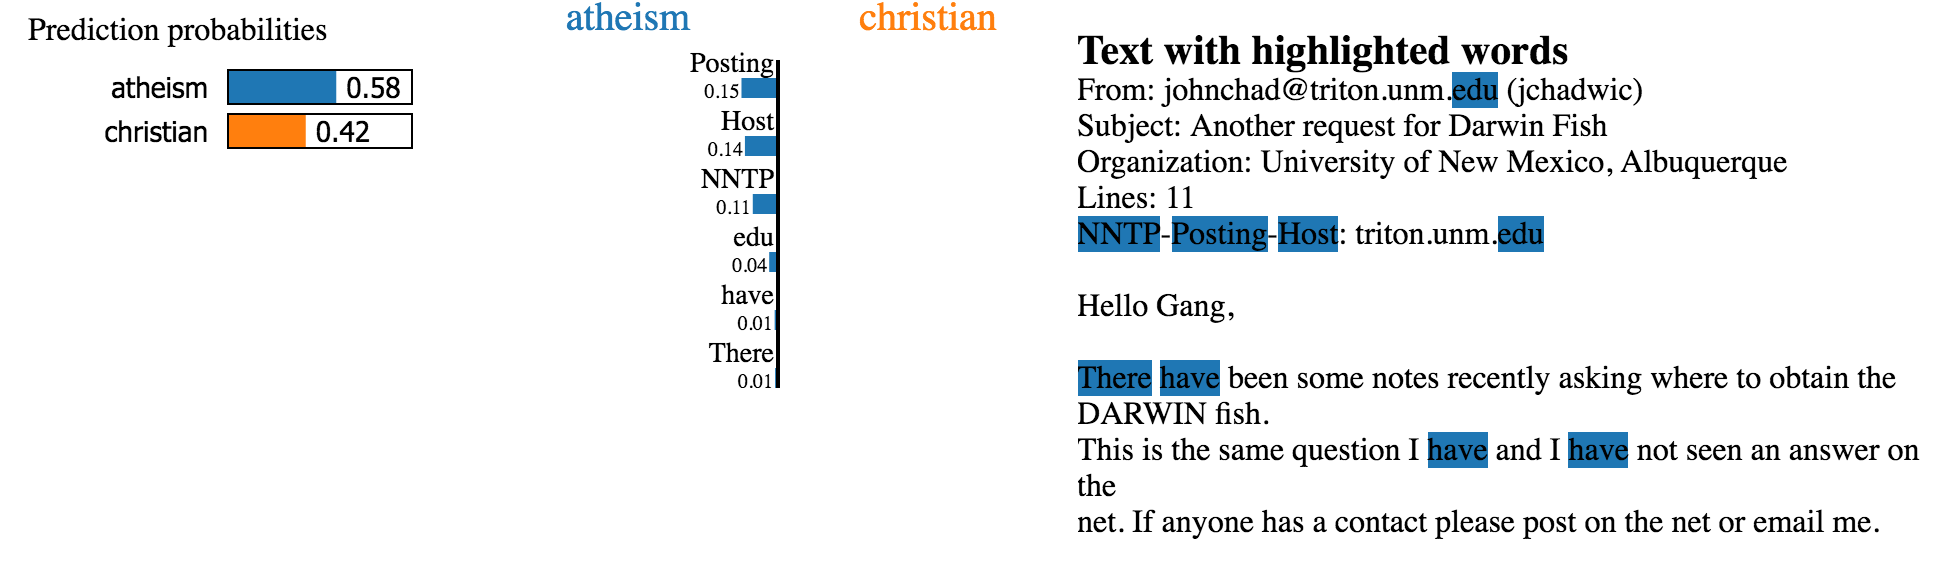
\includegraphics[width=0.83\textwidth,height=0.40\textheight,keepaspectratio]{images/responsible-ai/lime_text_twoclass_explanation.png}

    \vspace{0.3em}
    {\scriptsize Source: \texttt{lime} library documentation,
    \href{https://github.com/marcotcr/lime}{github.com/marcotcr/lime}
    (\texttt{doc/images/twoclass.png}); 20 Newsgroups atheism-vs-christianity classifier.}

    \vspace{0.5em}
    \raggedright
    \begin{itemize}\small
        \setlength\itemsep{0.3em}
        \item The classifier reports 0.58 for ``atheism.'' The explanation shows the evidence:
              \texttt{Posting}, \texttt{Host}, \texttt{NNTP}, \texttt{edu} --- \textbf{email header
              artefacts}, not content.
        \item This is the single most valuable use of local explanations: a high-accuracy model
              that is right for a reason that will not survive contact with new data.
        \item You would never have found it from the accuracy score.
    \end{itemize}
\end{frame}

\begin{frame}{LIME on Images}

    \centering
    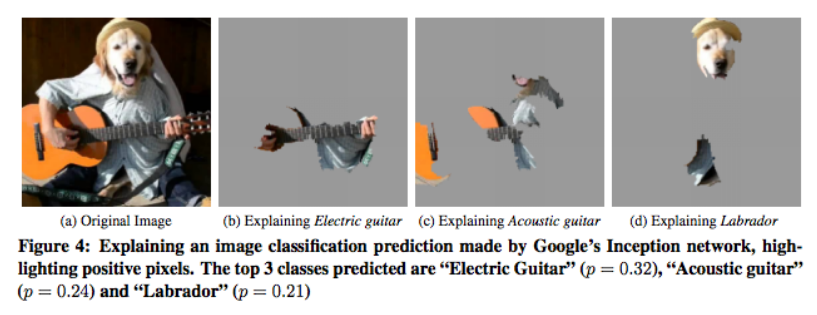
\includegraphics[width=0.78\textwidth,height=0.40\textheight,keepaspectratio]{images/responsible-ai/lime_paper_fig4_image_explanations.png}

    \vspace{0.3em}
    {\scriptsize Source: Figure 4 of M.~T.~Ribeiro, S.~Singh and C.~Guestrin, ``\,`Why Should I
    Trust You?': Explaining the Predictions of Any Classifier,'' KDD 2016
    (\href{https://arxiv.org/abs/1602.04938v3}{arXiv:1602.04938v3}), as reproduced in the
    \href{https://github.com/marcotcr/lime}{\texttt{lime}} repository.}

    \vspace{0.6em}
    \raggedright
    \begin{itemize}\small
        \setlength\itemsep{0.3em}
        \item The image is segmented into superpixels; perturbation switches groups of them off.
        \item Each panel shows the superpixels supporting a \emph{different} predicted class ---
              the explanation is always \textbf{relative to a target class}, never absolute.
        \item Useful check: if the supporting region is the background rather than the object, you
              have found a dataset artefact.
    \end{itemize}
\end{frame}

\begin{frame}[allowframebreaks]{Pitfalls You Must Know Before Using Either}

    \begin{itemize}
        \setlength\itemsep{0.5em}
        \item \textbf{Correlated features.} Both methods perturb features independently, producing
              rows that could not exist. Attribution then gets spread arbitrarily among correlated
              features, and can be assigned to a feature the model barely uses. Group correlated
              features and attribute to the group.

        \item \textbf{The background / neighbourhood is a choice.} SHAP values are relative to the
              background dataset; LIME weights depend on the kernel width and the perturbation
              scheme. Report what you used --- otherwise the numbers are not reproducible.

        \item \textbf{Instability.} Re-running LIME with a different seed can reorder the top
              features. Always run it several times and check the explanation is stable before
              you show it to anyone.

        \item \textbf{Explanations can be attacked.} Slack et al.\ (2020) built classifiers that
              behave in a biased way on real data but detect the synthetic perturbation
              distributions used by LIME and SHAP, and answer innocuously there --- so the
              explanation hides the bias.
    \end{itemize}

    \vspace{0.5em}
    \begin{block}{}
        \centering
        \small \textbf{Exercise} (companion notebook in preparation): run SHAP (Tree and
        Kernel) and LIME on the same tabular model, with an explicit demonstration of instability
        under correlated features.
    \end{block}

    \vspace{0.3em}
    {\scriptsize D.~Slack, S.~Hilgard, E.~Jia, S.~Singh and H.~Lakkaraju, ``Fooling LIME and SHAP:
    Adversarial Attacks on Post hoc Explanation Methods,'' AIES 2020,
    \href{https://arxiv.org/abs/1911.02508v2}{arXiv:1911.02508v2}.}
\end{frame}

\begin{frame}{Explaining the Model vs Explaining the World}

    \begin{columns}[T]
        \begin{column}{0.48\textwidth}
            \begin{tcolorbox}[colback=raiBlue!5, colframe=raiBlue!60, title=What SHAP answers]
                \scriptsize ``How does \emph{this fitted function} distribute its output across the
                inputs I gave it?''

                \vspace{0.12em}
                A statement about the model. Correct as far as it goes.
            \end{tcolorbox}
        \end{column}
        \begin{column}{0.48\textwidth}
            \begin{tcolorbox}[colback=raiRed!5, colframe=raiRed!70, title=What people hear]
                \scriptsize ``Which factors \emph{cause} this outcome, and what should this person
                change?''

                \vspace{0.12em}
                A causal statement. Not supported by the attribution.
            \end{tcolorbox}
        \end{column}
    \end{columns}

    \vspace{0.24em}

    \begin{itemize}\scriptsize
        \setlength\itemsep{0.1em}
        \item Kumar et al.\ (2020) argue that the mathematical appeal of Shapley values does not
              transfer to the human goals people bring to explanations, and that closing the gap
              requires causal assumptions the method does not make.
        \item If the user needs \textbf{recourse} (``what do I change?''), the right tool is a
              \textbf{counterfactual explanation} --- the nearest feasible input that flips the
              decision --- not a feature attribution.
        \item \textbf{Not unique, and not a defence.} Different methods, backgrounds and seeds give
              different attributions for the same prediction; a reviewer finding an explanation
              satisfying is not evidence the model is correct.
        \item \textbf{Rule of thumb:} use explanations to \textbf{generate hypotheses}, then test
              each one by intervention --- an ablation, a re-fit without the feature, a fresh slice.
    \end{itemize}

    \vspace{0.09em}
    {\scriptsize I.~E.~Kumar, S.~Venkatasubramanian, C.~Scheidegger and S.~Friedler, ``Problems with
    Shapley-value-based explanations as feature importance measures,'' ICML 2020,
    \href{https://arxiv.org/abs/2002.11097v2}{arXiv:2002.11097v2}.}
\end{frame}

